\chapter{Seasonal variation of atmospheric neutrino event rates}
\label{sec:seasonal}

Proper modeling of background data (especially with respect to time) is tantamount to successful short timescale analyses. Although to first order, background distributions seem independent of time, there is known underlying oscillatory structure at the $\mathcal{O}(10\%)$ level due to changes in atmospheric conditions, which affect atmospheric lepton production rates from cosmic-ray interactions. Many current analyses do not take this \textit{seasonal variation} into account, and those that do have treated the rate as a one-dimensional sine wave in time affecting the rate of the entire sample. Here, we investigate if this is a proper treatment. 

We begin with the assumption that we are working with a finite viewing window of a sinusoidal rate, $\mathcal{R}$\footnote{here, $\mathcal{R}$ is only the fluctuation from the mean rate, $\mathcal{R} = \frac{r-<r>}{<r>}$, where $r$ is the true rate}:

\begin{equation}
\label{eq:rate}
    \mathcal{R}(f,t,\delta, w) = \Pi \left(\frac{t-\pi  w}{2 \pi  w}\right) \sin (2 \pi  \delta +f t) \; , 
\end{equation}

where $t$ is the time, $f$ is the frequency, $\delta$ is an offset, and our viewing window is encompassed by a unit step function, $\Pi$, with width characterized by $w$. 

We are interested in observing this rate in frequency space, and naturally wish to take a Fourier Transform (FT). We will apply this procedure to our rate as a function of time, but also try to account for structures that should manifest in the FT from known imperfections in these data. In general, the FT of a function of time is given by

\begin{equation}
\label{eq:FFT}
    \mathcal{F}_t[\mathcal{R}(t)](\omega ) = \frac{1}{\sqrt{2 \pi}} \int_{-\infty}^{\infty} \mathcal{R}(t) e^{i \omega t} d t \; .
\end{equation}

We know that in the case of a pure sinusoid, the $\mathcal{F}$ operator should return delta functions corresponding to the frequency of our rate. This is also the case for an infinite viewing window,

\begin{equation}
    \lim_{w\rightarrow \infty} \mathcal{F}_t[\mathcal{R}(t)](\omega ) = i \sqrt{\frac{\pi }{2}} e^{-2 i \pi  \delta } \delta (\omega -f)-i \sqrt{\frac{\pi }{2}} e^{2
   i \pi  \delta } \delta (f+\omega ) \; .
\end{equation}

One immediate problem is that we have limited years of data, so we begin by investigating the effect that a limited viewing window has on our FT. Applying Eq.~\ref{eq:FFT} to our rate function defined in Eq.~\ref{eq:rate}, and taking the magnitude in $\mathbb{C}$, we get 

\begin{multline}
   \mathcal{F}_t[\mathcal{R}(t)](\omega ) =  \Bigg| \frac{1}{4\pi (f^2 - \omega^2)}(\theta (-w)-\theta (w)) (\cos (2 \pi  (\delta +f w-w \omega ))-i \sin (2 \pi  (\delta +f w-w
   \omega ))) \; \times \\ \qquad (2 i (f-\omega ) \sin (\pi  w (f+\omega )) (\cos (4 \pi  \delta +3 \pi  f w-\pi
    w \omega )+i \sin (4 \pi  \delta +3 \pi  f w-\pi  w \omega )) \; +  \\ (-f-\omega ) (i \sin (2 \pi
    f w-2 \pi  w \omega )+\cos (2 \pi  f w-2 \pi  w \omega )-1)) \Bigg| \; ,
\end{multline}

which can be simplified to 

\begin{multline}
    \mathcal{F}_t[\mathcal{R}(t)](\omega ) = \frac{1}{4\pi} \Big| \frac{1}{f^2 - \omega^2} \Big( e^{- 2 \pi i (fw+\delta-w\omega)}\big(-(f+\omega)(-1+e^{2\pi i w(f-\omega)}) + \\ 2i\sin (\pi w(f + \omega)) e^{i(3f\pi w + 4\pi \delta - \pi w \omega)}\big) \Big) \Big|
\end{multline}

A sample time series and the corresponding FT are displayed in Fig.~\ref{fig:ex_fft}. Here, the effect of the finite viewing window is visible in the separate peaks in the FT, a consequence often referred to as \textit{spectral leakage}\footnote{For a thorough writeup on spectral leakage, see \url{https://en.wikipedia.org/wiki/Spectral_leakage}.}.
\begin{figure}
    \centering
    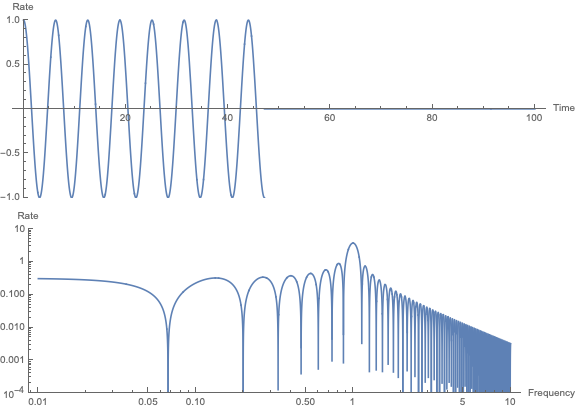
\includegraphics[width=0.90\textwidth]{figures/seasonal/box_fft_sample.png}
    \caption[Windowing effect in FFTs]{A sample time series (top) with a pure sine wave and finite viewing period (7.5 cycles) with corresponding FT (bottom)}
    \label{fig:ex_fft}
\end{figure}
%In the gamma-ray followup (GFU) dataset, it has been noted in the past that the effects of seasonal variations are evident, and manifest in an overall $\mathcal{O}$(10\%) fluctuation in the background rate. 
%For short timescale analyses, an accurate prediction of the background rate is of utmost importance in quantifying the significance of a possible signal. As a result of seasonal variations, calculating the rate from the entire livetime of the dataset leads to systematic over- and under-estimations of the rate, whereas parameterizing the background rate from data around the time of a transient event is limited by statistical fluctuations of the rate. In order to see if we can model the rate as a sinusoid, we take an FFT of the rate data, and try to make sure that any features can be explained by what is expected from an FFT of a windowed sinusoid.

\begin{figure}
    \centering
    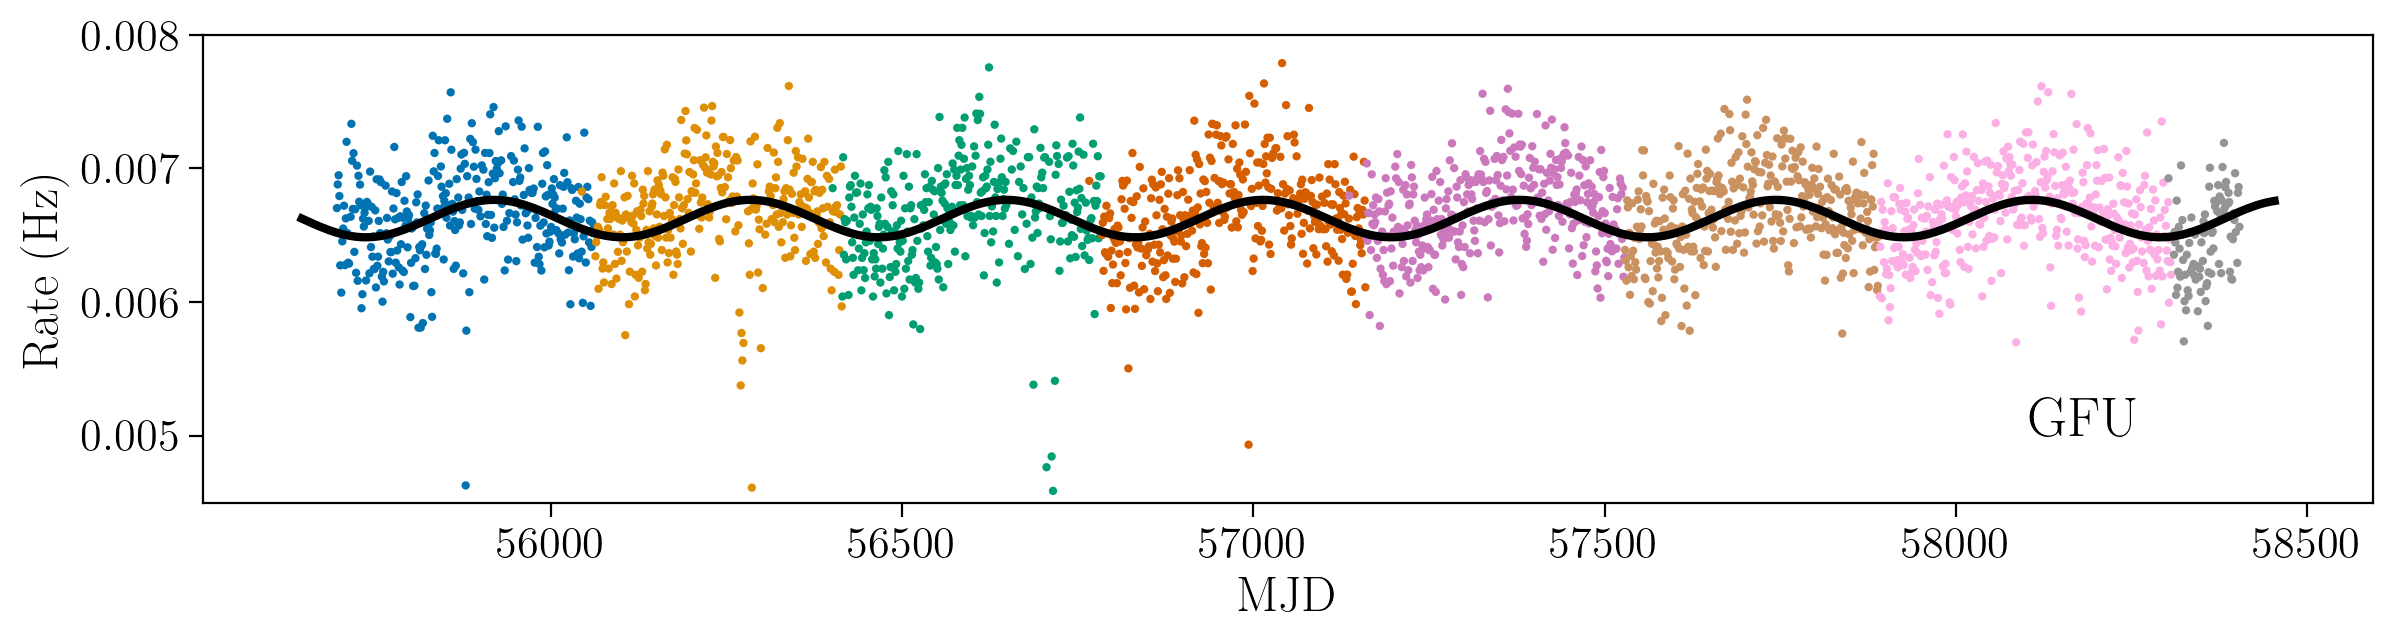
\includegraphics[width=0.9\textwidth]{figures/seasonal/gfu_online_overall_with_model.png}
    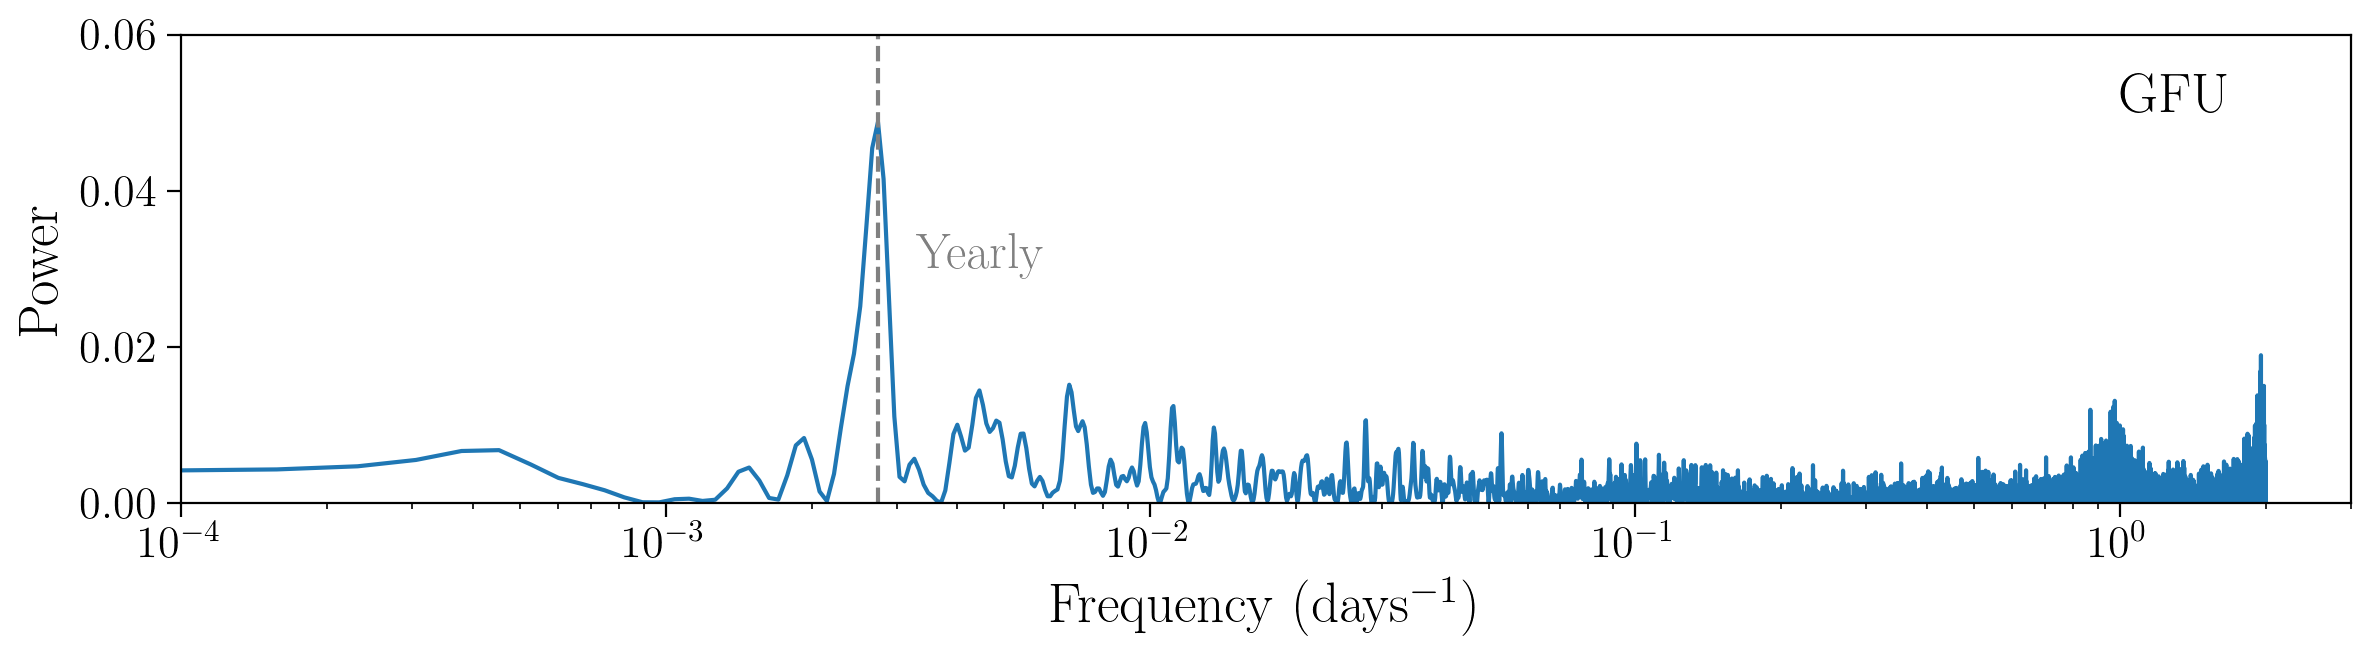
\includegraphics[width=0.9\textwidth]{figures/seasonal/gfu_online_overall_FFT_maxima_False.png}
    \caption[GFU all sky rate]{GFU time series (top) and FT (bottom) for 7.5 years of data. Each color is a different season of IC86 data.}
    \label{fig:gfu_7_year_fft}
\end{figure}

Fig.~\ref{fig:gfu_7_year_fft} shows the rate time series and corresponding FT for the 7.5 years of available data from GFU. Here, as the data is sampled unevenly, we use the Lomb-Scargle periodogram\footnote{For details on the algorithm, see \url{https://arxiv.org/abs/1703.09824}.} algorithm to transform these data into frequency space. There is clear structure to the left of the annual peak. To investigate if these are the expected peaks, we extremize numerically, and find that there should be peaks at frequencies of $\{0.41,0.54,0.67,0.8\}\times f_0$, where $f_0$ is the peak frequency in the plots in the figures above. The numerical derivative has some odd structure, and is displayed in Fig.~\ref{fig:fft_derivative}.

\begin{figure}
    \centering
    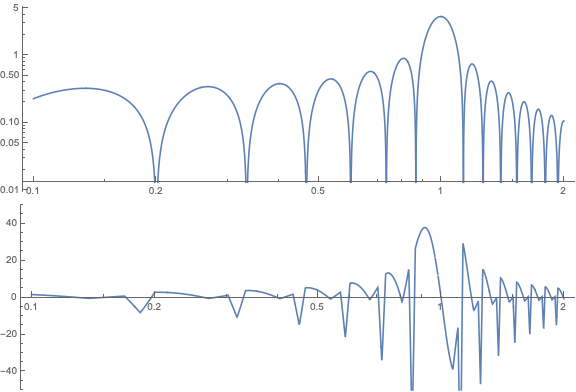
\includegraphics[width=0.75\textwidth]{figures/seasonal/GFU_fft_with_derivative.png}
    \caption[Numerical derivative of FFT of windowed data]{FT (top) and numerical derivative of FT (bottom)}
    \label{fig:fft_derivative}
\end{figure}

Looking at other durations and doing a crude fit, it seems as though the maxima appear at roughly $f_0 + (\frac{3}{2} + n)\frac{1}{w}$, where $n = 0,1,2,\ldots$
Placing lines at the corresponding frequencies in the GFU FT results in Fig.~\ref{fig:gfu_with_harmonics}

\begin{figure}
    \centering
    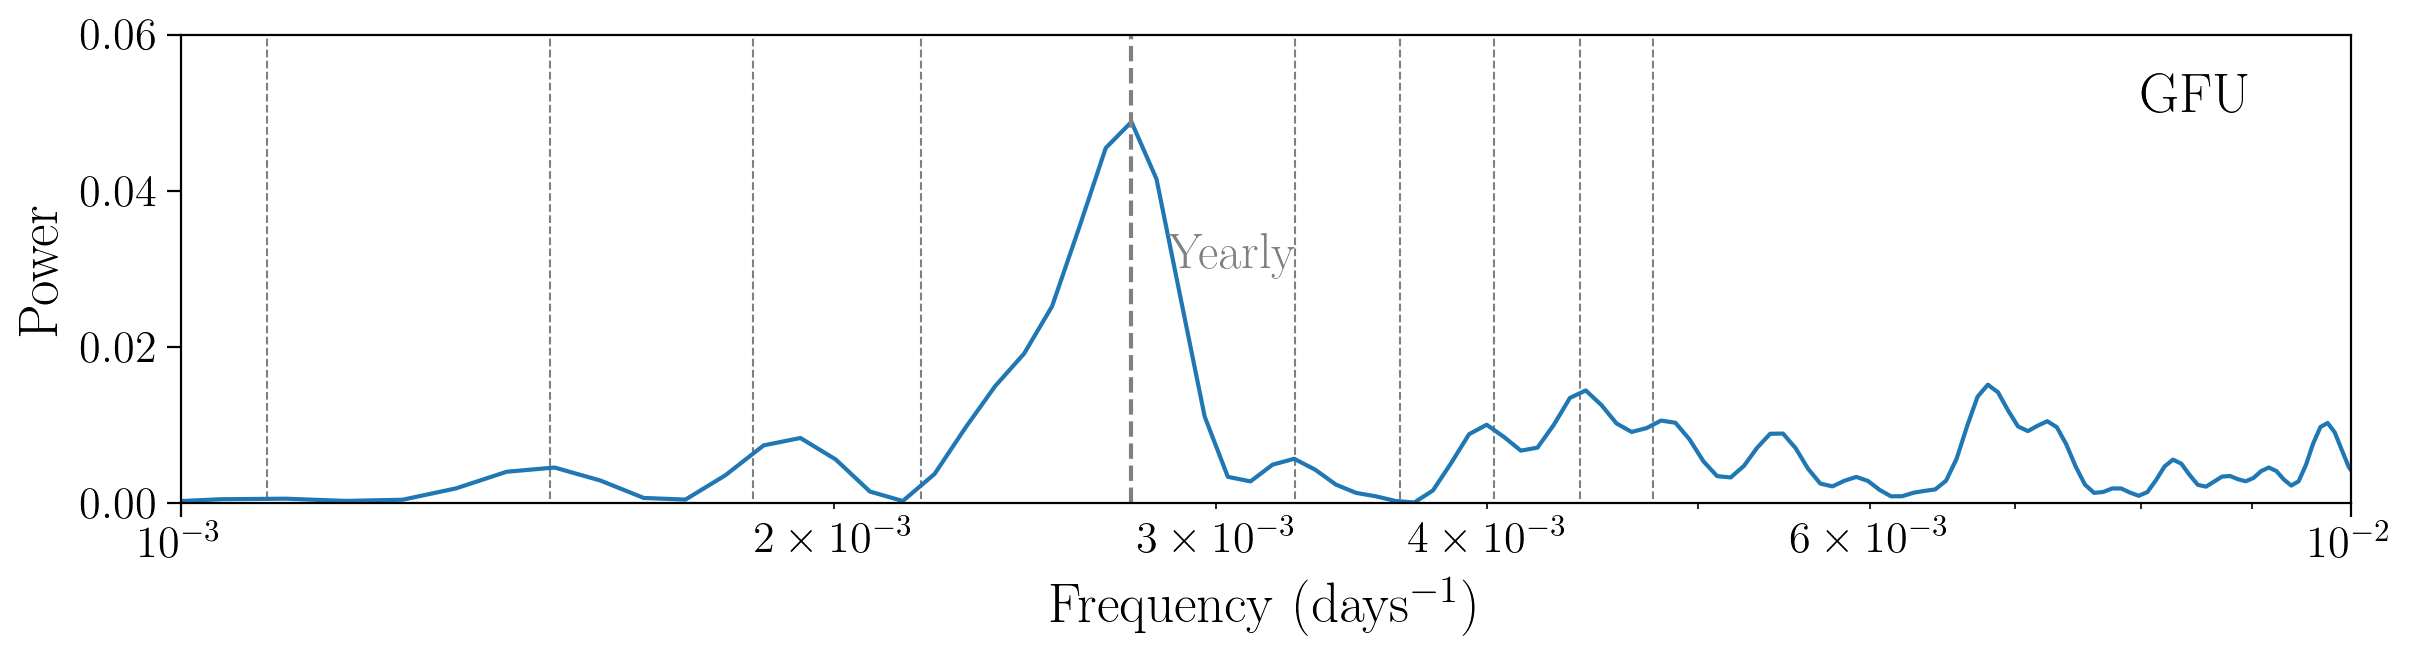
\includegraphics[width=0.95\textwidth]{figures/seasonal/gfu_online_overall_FFT_maxima_True.png}
    \caption[FFT numerical derivative]{GFU FT with additional lines at the locations of the extremal frequencies extracted from Fig.~\ref{fig:fft_derivative}}.
    \label{fig:gfu_with_harmonics}
\end{figure}

\section{Declination Dependence}
Seasonal variations are mainly a function of atmospheric properties. As the temperature and pressure of the atmosphere fluctuate, the ratio of the decay length to interaction length for $\pi^{\pm}$ created from cosmic-ray interactions will vary. As such, the the magnitude of the seasonal variation effect is dependent on zenith angle, $\theta$ (plots shown here are for Equatorial coordinates shown in slices of equal solid angle, or equal $\sin \delta$). 

We begin by repeating the procedure of the previous section, but in various declination bands. The result is shown in Fig.~\ref{fig:dec_bands}.

\begin{figure}
    \centering
    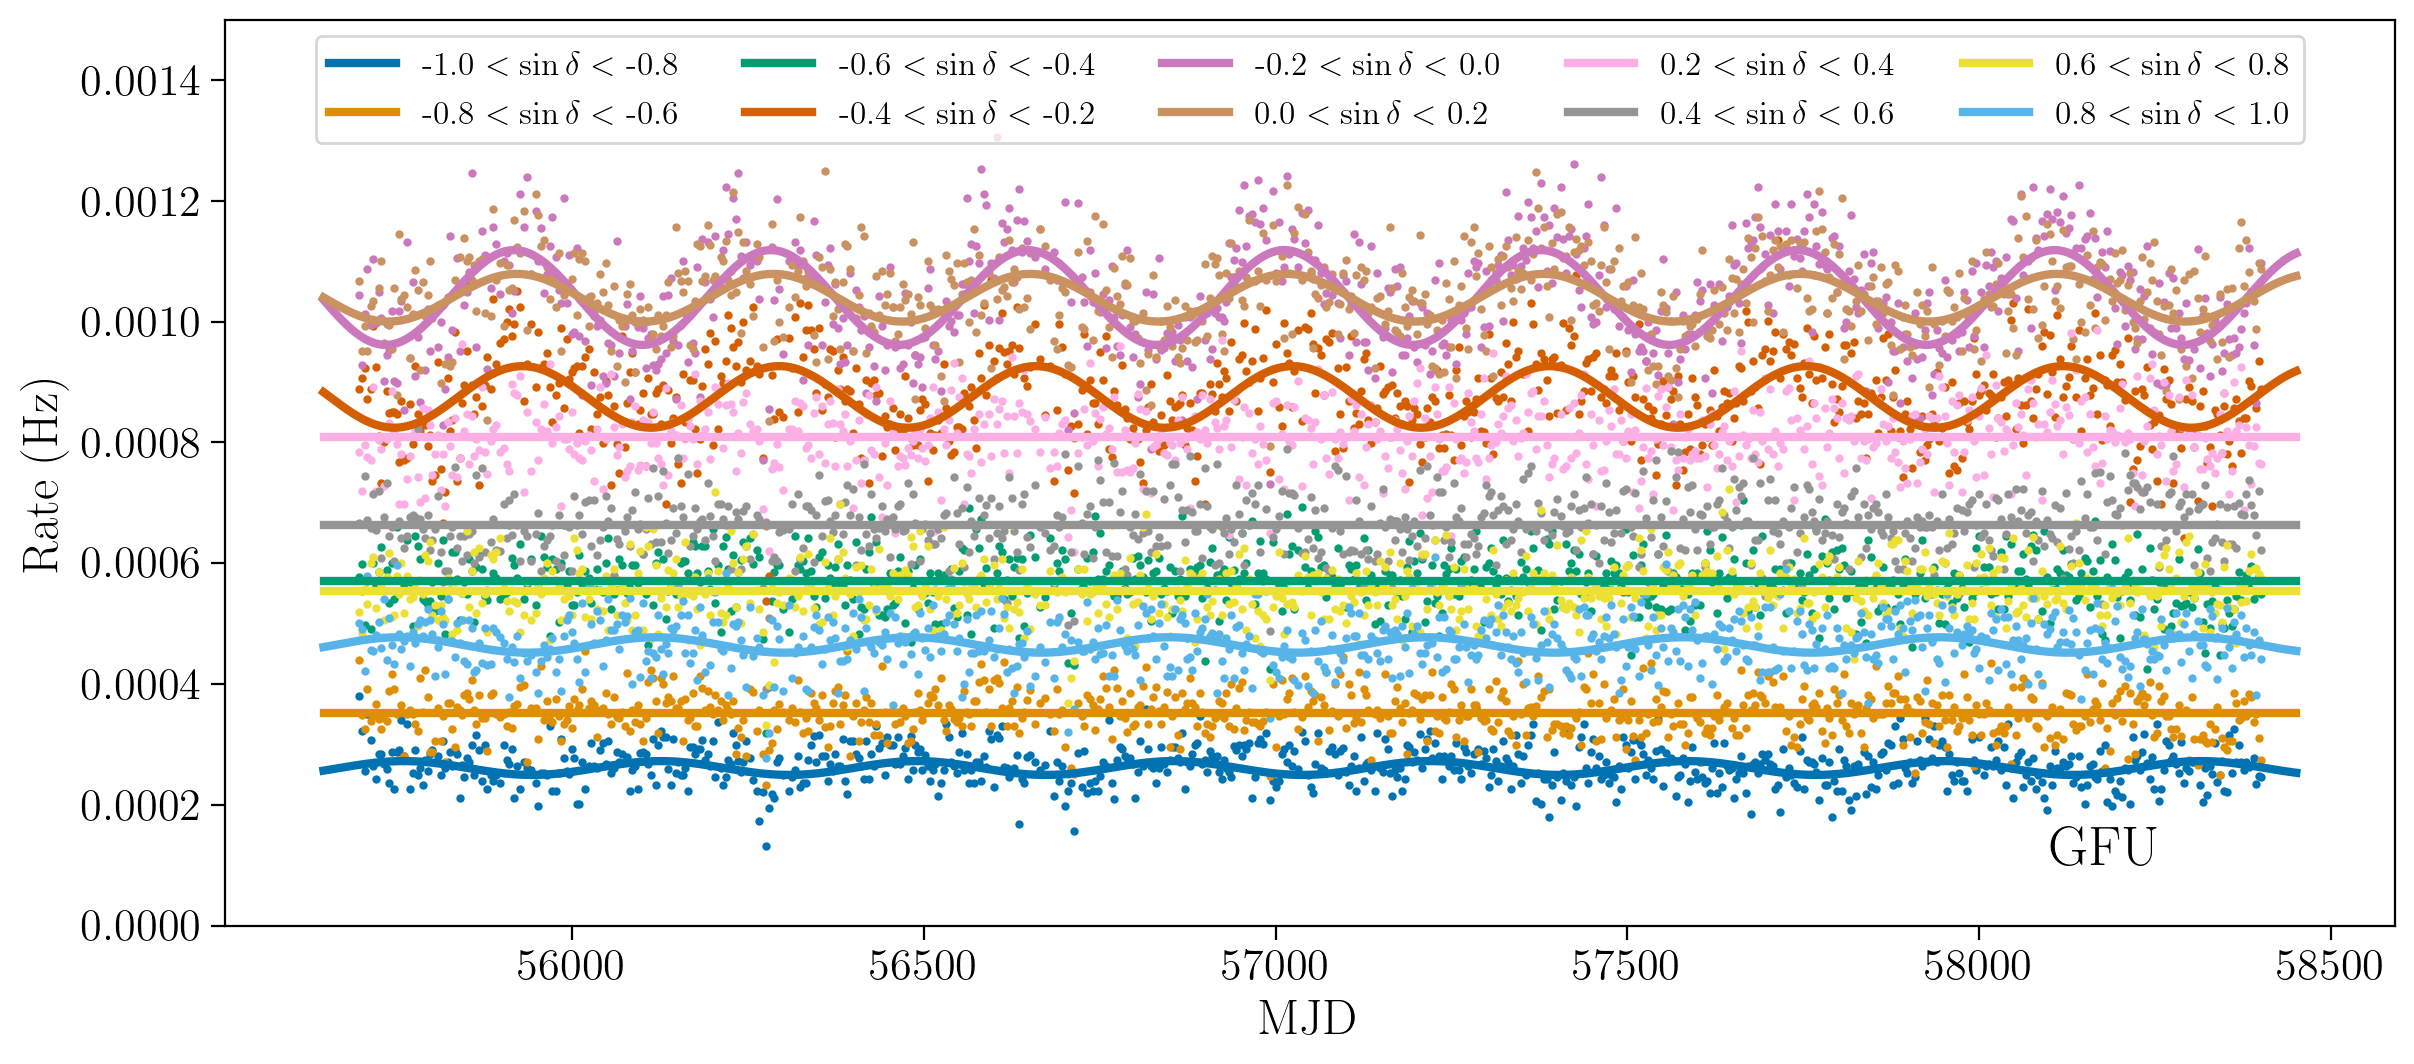
\includegraphics[width=0.99\textwidth]{figures/seasonal/gfu_online_dec_band_with_model.png}
    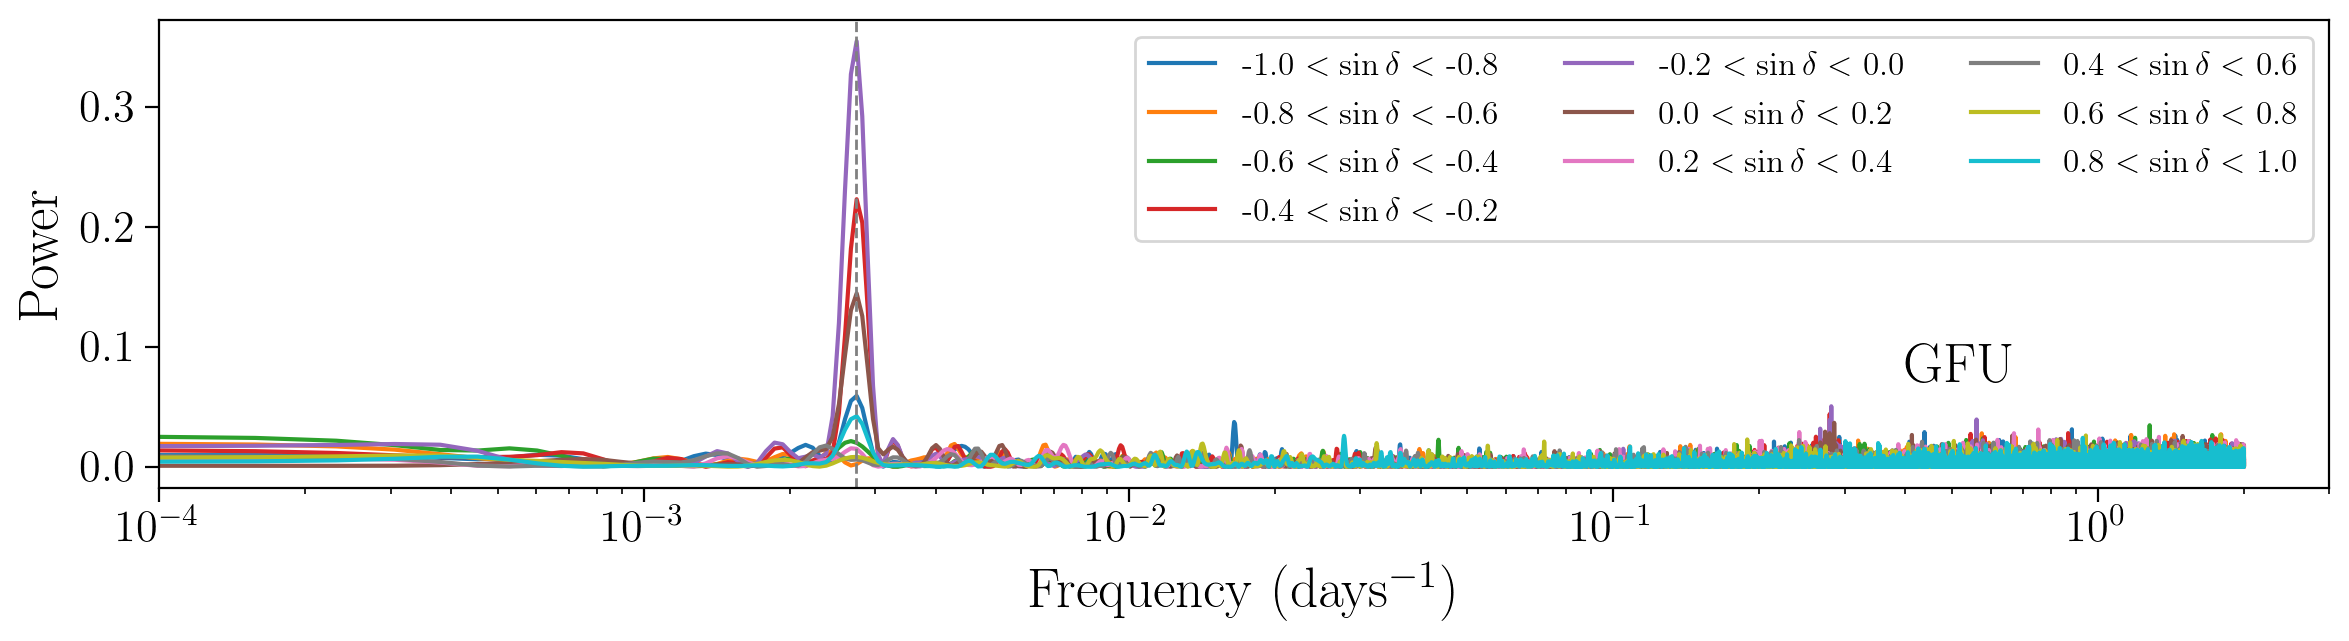
\includegraphics[width=0.99\textwidth]{figures/seasonal/gfu_online_dec_bands_FFT.png}
    \caption[\texttt{GFU} seasonal variations]{Rate as a function of time for various declination bands (top). Fits are only included if the p-value of the annual structure in the FT is at or below the 1\% level. FT (bottom) highlights that seasonal variations are more evident in certain declination bands}
    \label{fig:dec_bands}
\end{figure}

Although seasonal variations are expected in all samples, the magnitude of the effect varies from sample to sample, depending on how contaminated the sample is with atmopherics. See for example by comparing the frequency dependence of the GFU sample to that of the ps-tracks sample, which is shown in Fig.~\ref{fig:dec_bands_ps_tracks}.

\begin{figure}
    \centering
    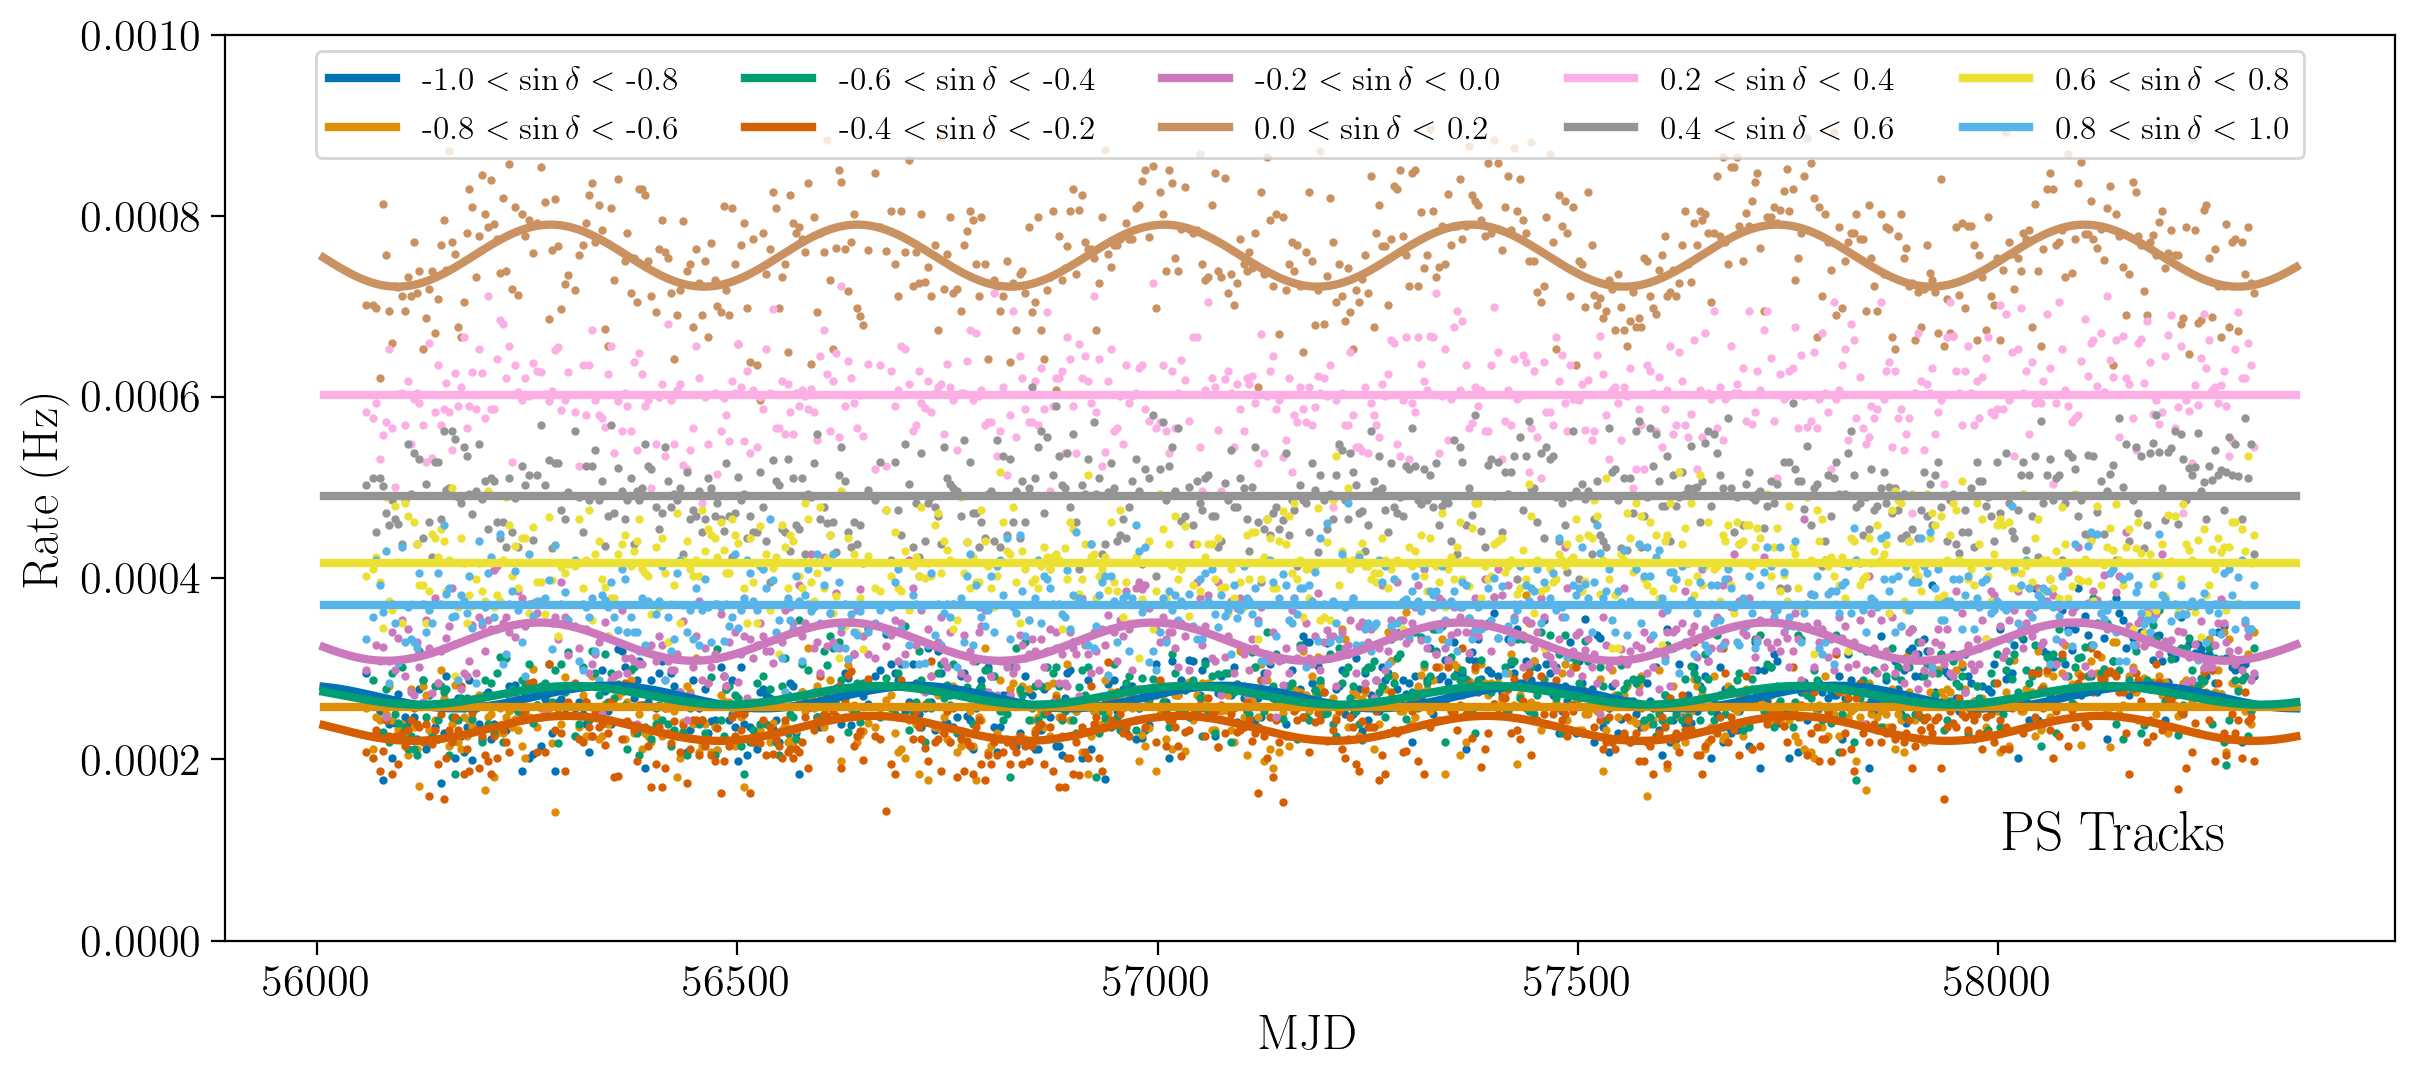
\includegraphics[width=0.99\textwidth]{figures/seasonal/ps_tracks_dec_band_with_model.png}
    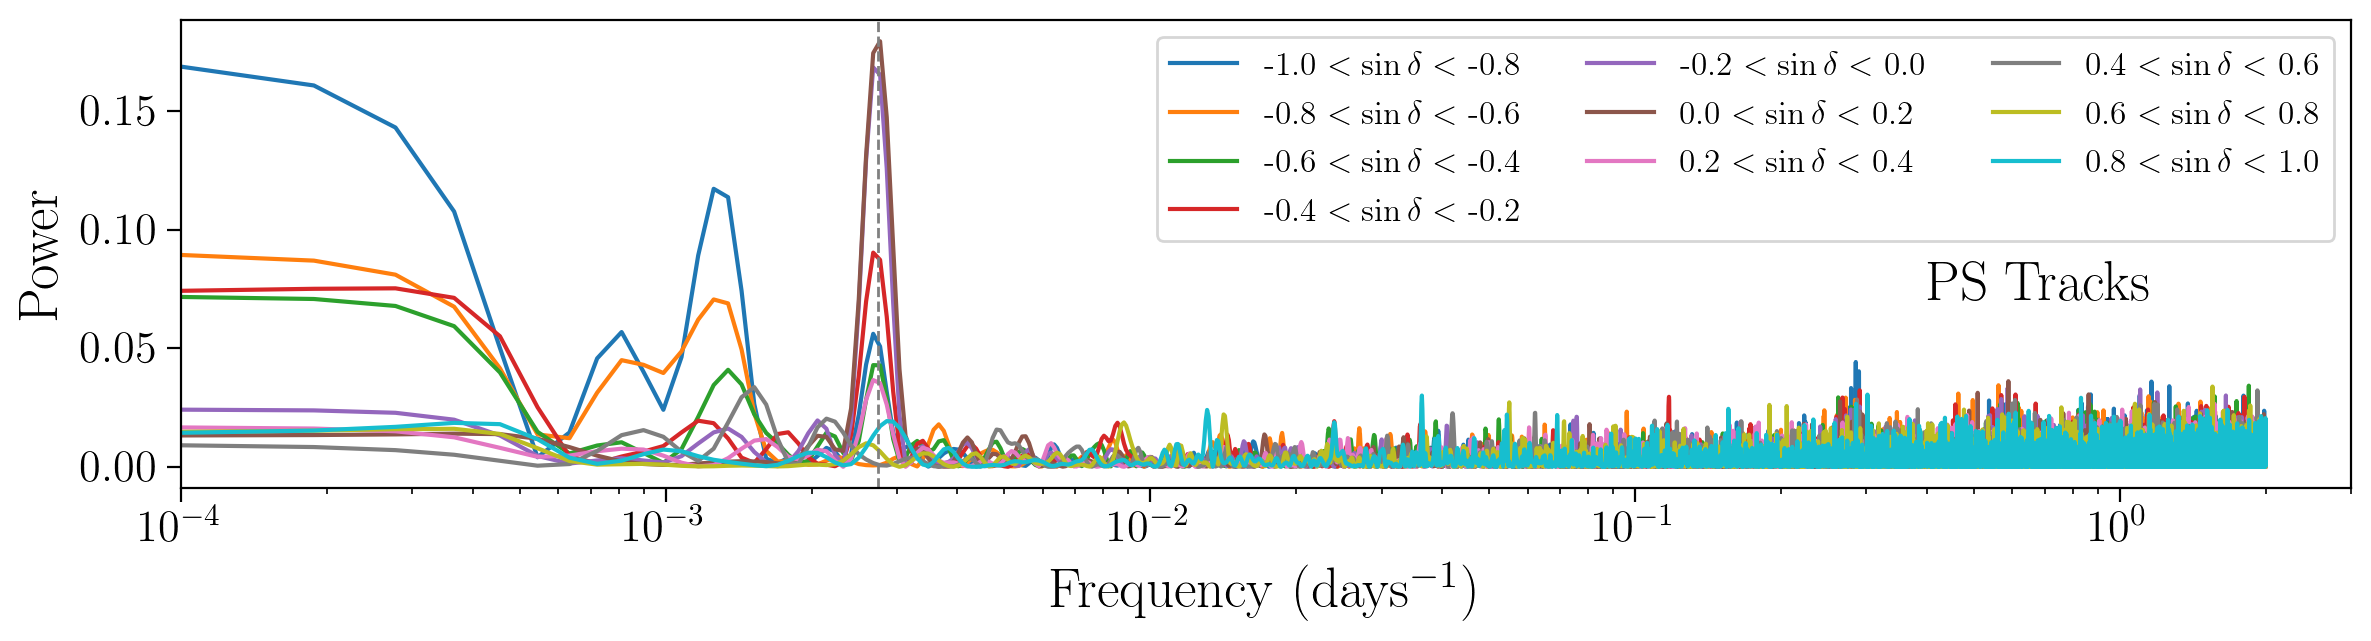
\includegraphics[width=0.99\textwidth]{figures/seasonal/ps_tracks_dec_bands_FFT.png}
    \caption[\texttt{ps-tracks} seasonal variations]{The same as Fig.~\ref{fig:dec_bands} but for the \texttt{ps-tracks} sample.}
    \label{fig:dec_bands_ps_tracks}
\end{figure}

Instead of looking at the FTs in terms of the power in each frequency, one can also look at the amplitude (in units of the rate, and thus not normalized to the rate in each declination band). We display these as vectors in a 2D plane for both event selections, shown in Fig.~\ref{fig:phasor}. 

\begin{figure}
    \centering
    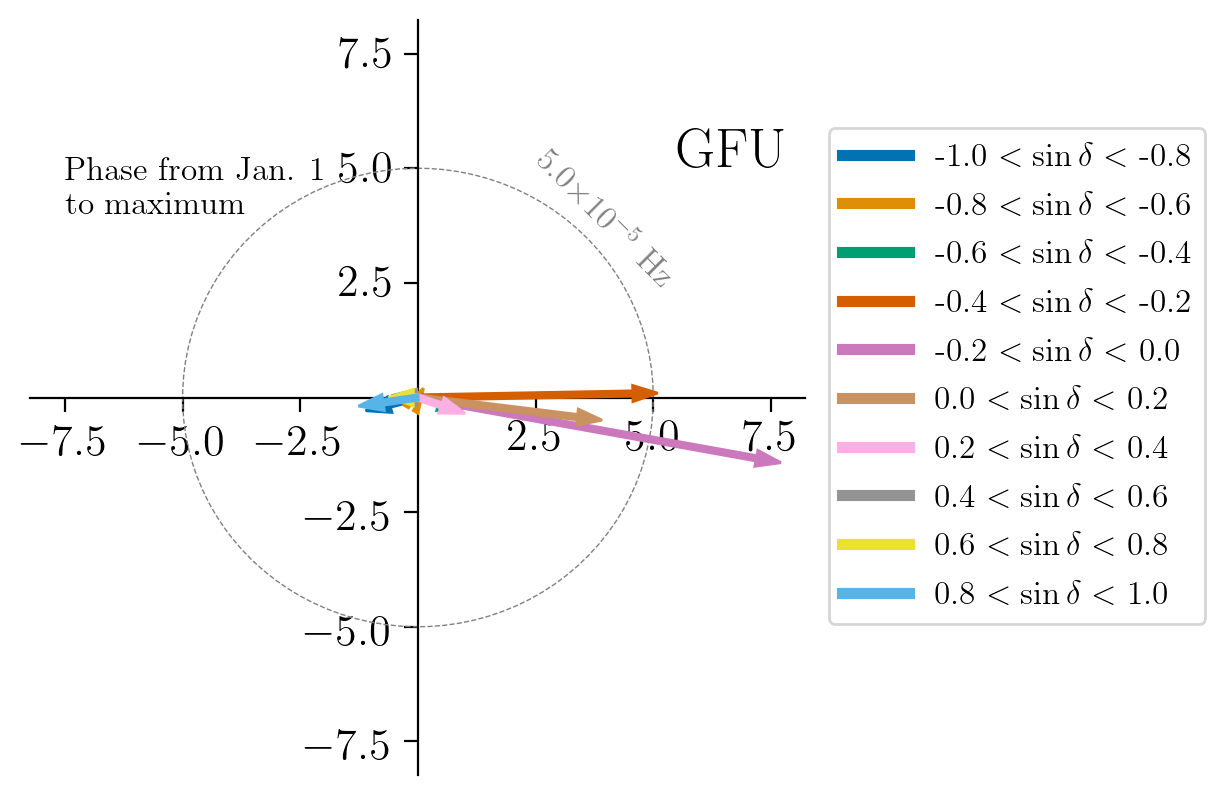
\includegraphics[width=0.48\textwidth]{figures/seasonal/gfu_online_phasor.png}
    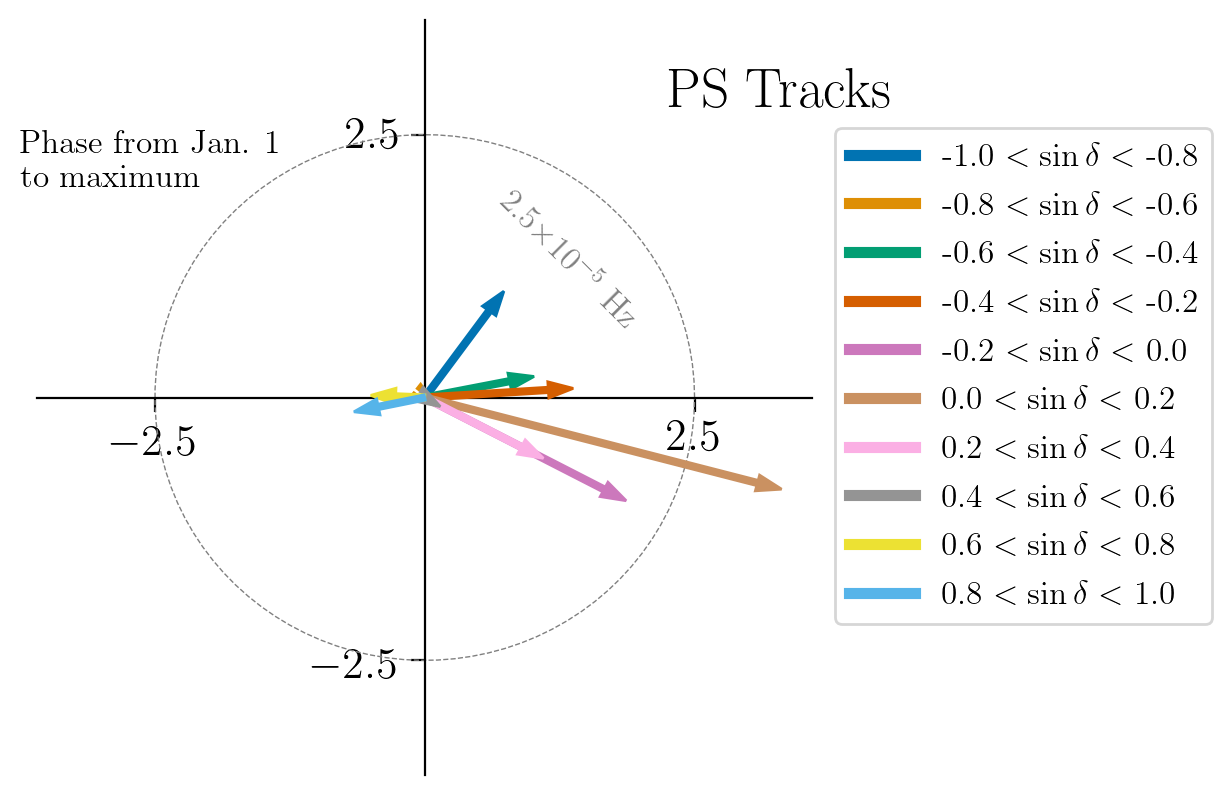
\includegraphics[width=0.48\textwidth]{figures/seasonal/ps_tracks_phasor.png}
    \caption[Seasonal variation phasors]{Phases and amplitudes of the annual peak in the FT broken down by declination band. For different zenith angle bands, the phases of the sinusoids are out of phase, in some cases nearly 180$\deg$. }
    \label{fig:phasor}
\end{figure}

Phases in Fig.~\ref{fig:phasor} are shown as the phase from Jan. 1 to the phase of maximal amplitude, as shown by the schematic in Fig.~\ref{fig:ft_schematic}. 

\begin{figure}
    \centering
    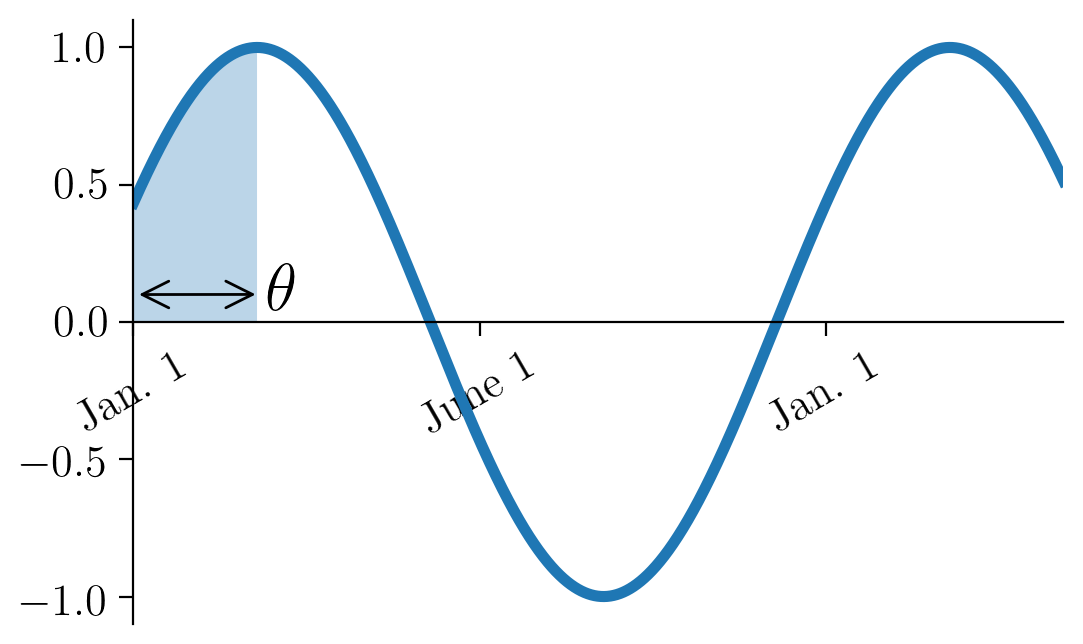
\includegraphics[width=0.55\textwidth]{figures/seasonal/phase_schematic.png}
    \caption[Phase convention schematic]{Definition of the phases for Fig.~\ref{fig:phasor}.}
    \label{fig:ft_schematic}
\end{figure}

As both the relative and absolute magnitudes, as well as the phase information, are important, we plot all three as a function of declination, here only focusing on the GFU dataset. The result is shown in Figure~\ref{fig:seasonal_3panel}. 

\begin{figure}
    \centering
    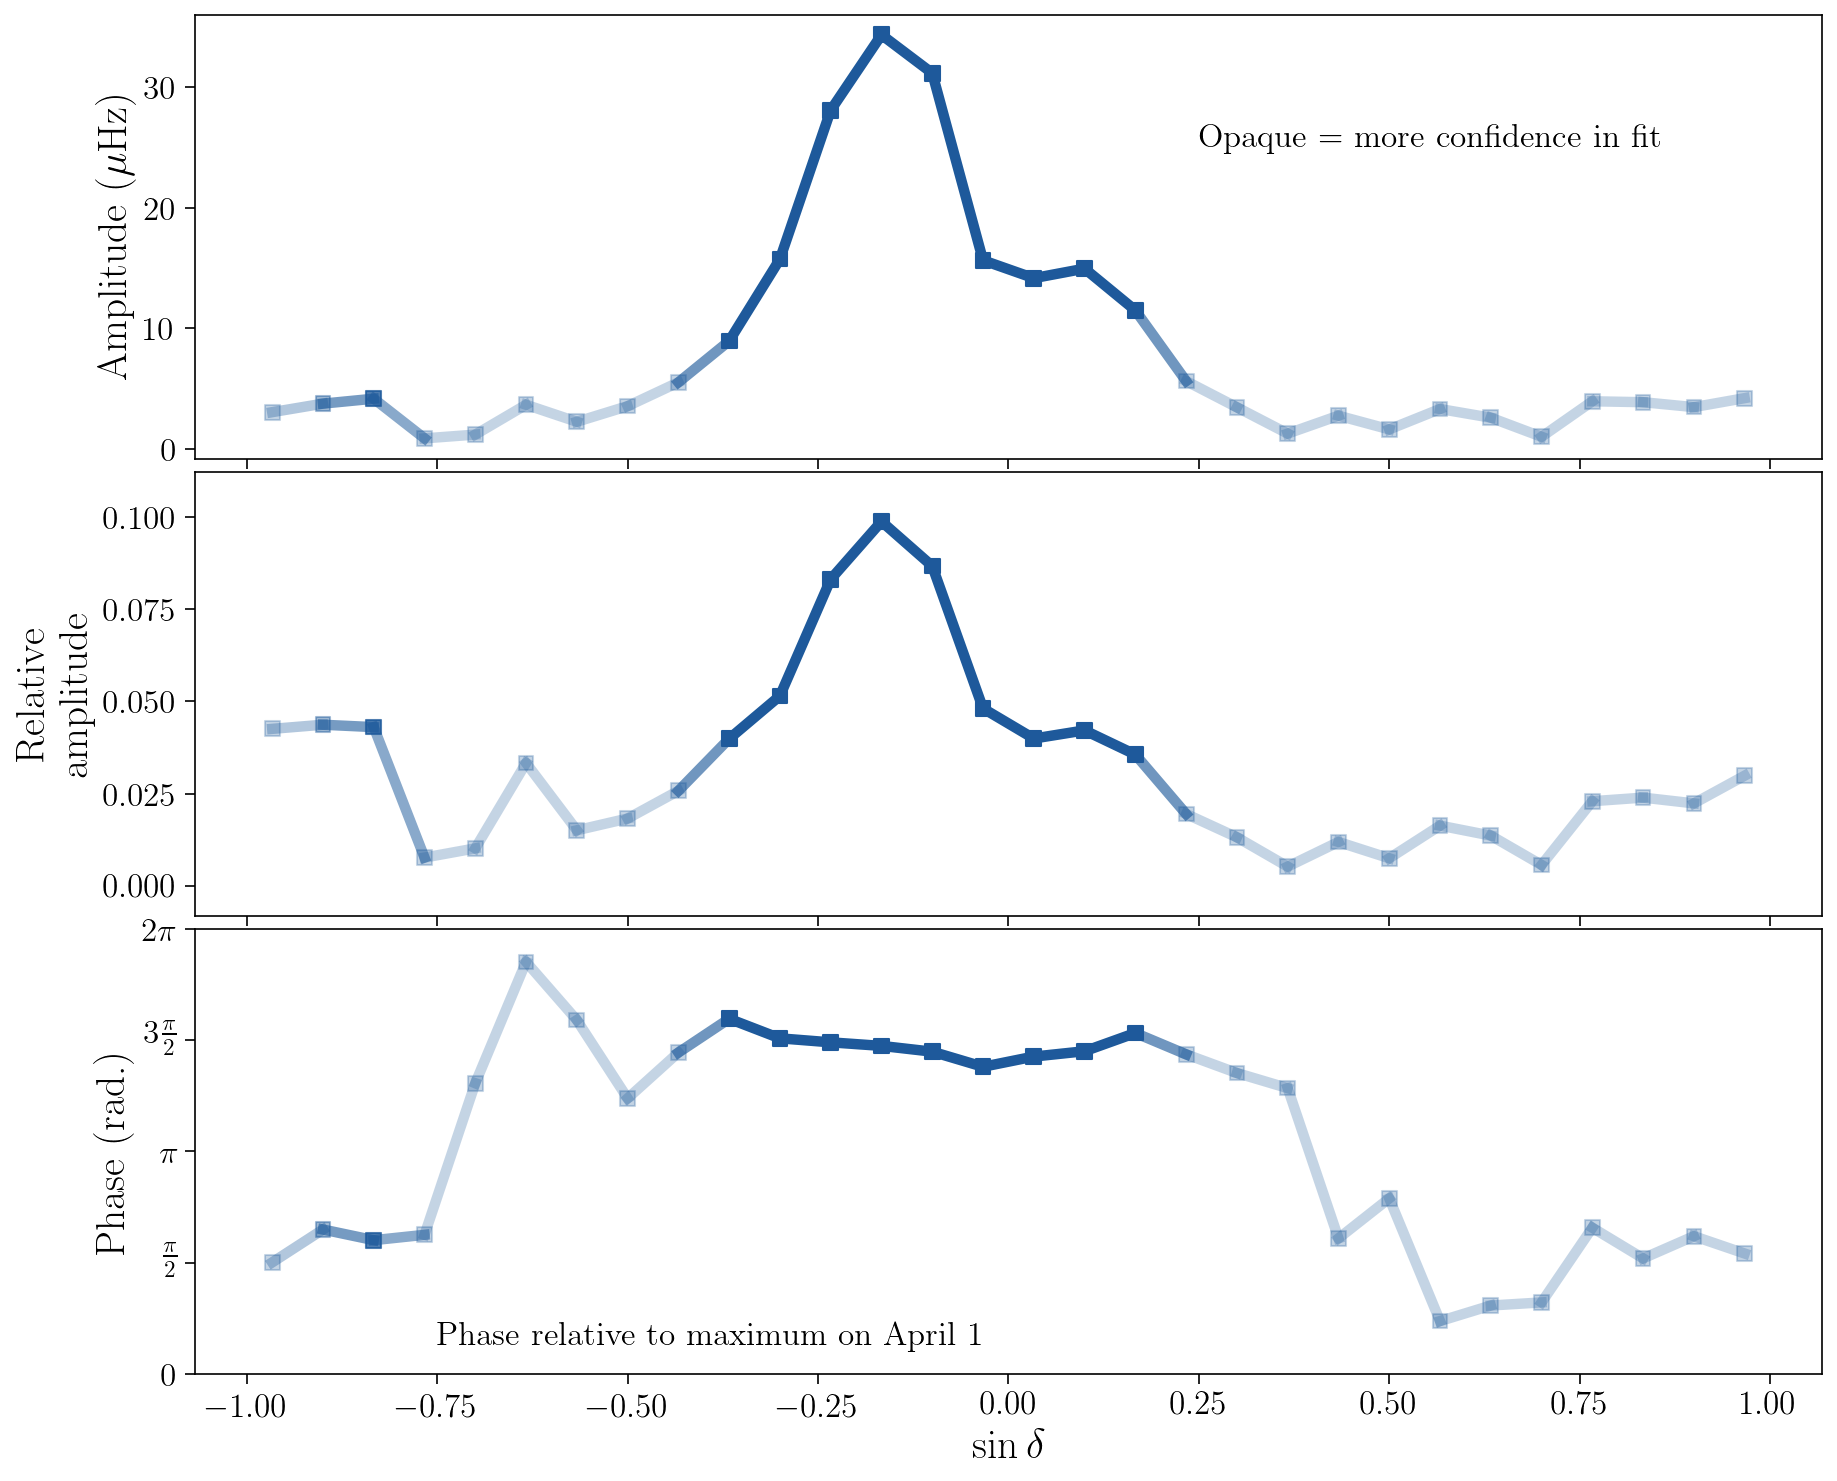
\includegraphics[width=0.95\textwidth]{figures/seasonal/seasonal_3panel_plot.png}
    \caption[Absolute and relative fourier component magnitudes]{Evolution of the absolute magnitude (top), relative magnitude (middle), and phase (bottom) of the annual sinusoidal component in the GFU event sample rate. Data points that appear transparent are regions where the sinusoidal fit was not preferred strongly over a constant rate. Regardless, the amplitudes still display a clear pattern as a function of declination, peaking near the horizon as one would expect.}
    \label{fig:seasonal_3panel}
\end{figure}

Although in some declination bands, the sinusoidal component is not dominant enough to be fit confidently, there is still a clear trend in the effect as a function of declination. 